
\section{Analysis}\label{analysis}

We now present our determinations of whether published detections of group
polarization are plausibly spurious and calculate the best-case false detection
rate for each experimental design in the corpus. We found that 95\% of all
detections of group polarization are plausibly false, 54 out of 57. We estimate the
best-case median false detection rate to be 72\% for those 54 experimental
conditions. All but seven of the 54 designs were found to require a $d^* > 0.8$
for ``significant'' Cohen's $d$ to limit the family-wise error rate to 5\%.


\subsection{Nearly all group polarization detections are plausibly spurious}


% We used our formal distribution model of group polarization experiments
% to identify plausible latent simple consensus distributions that generate spurious
% group polarization in 
Of the remaining 57, we identified simple consensus $\nu$ that generate spurious
group polarization in 54 experimental conditions. In the other three, we did
identify $\nu$ that generate spurious group polarization, but the initial
simulated distributions were highly polarized. 
We rejected $\nu$ generated for
two spurious group polarization from Schkade, et al., (2010) because
the histogram plots of the observed opinion distributions are not
polarized~\cite[Figure 1, p. 234]{Schkade2010}. The other condition where we
found but rejected spurious group polarization $\nu$ was in a question 
about a ``bad teacher'' in Myers (1975)~\cite{Myers1975a}, where lower values
signify increasingly worse impressions of the teacher and higher values signify
increasingly good impressions. It is unlikely that a
``bad teacher'' would be rated as good in this case, so we excluded this 
from our analysis as well. This exclusion may be overly generous since Myers (1975)
did not provide details beyond mean values and opinion shifts, and the article was
published before open data practices. Our corpus had a total of 60 experimental conditions, but we excluded 3 out of 60 
that did not claim to be positive findings of group polarization.

- Address sigmas, note differences

\begin{figure}
  \centering
    \includegraphics[width=\textwidth]{Figures/3.1/latent-sd-cdf.png}
    \caption{\textbf{}}
  \label{fig:}
\end{figure}



\subsection{Half of experiments exceed a 70\% false discovery rate at ``medium'' significance}

We simulated trials from each experimental condition, $e$, by sampling and binning
pre- and post-deliberation latent opinions from distributions with parameters
identified with the $N\to\infty$ model as causing plausibly spurious group
polarization. For each $e$, we drew a number of samples equal to the number of
participants in the original experiments, $N_\mathrm{emp}$. To estimate family-wise
error and false detection rates, we fit an ordered probit model to the simulated
observations and obtained estimates of the group polarization effect size, $d$
(Equation~\ref{eq:cohens}). If the effect size was greater than a significance
value, $d > d^*$, then by definition there was a detection $D$ of group
polarization, even though there was no effect by design, written $\neg E$.  The
family-wise error rate is $\Pr(D|\neg E)$, calculated as the frequency with which $d
> d^*$ out of 1000 simulation trials. The false detection rate is the family-wise
error rate scaled using the base rate of effects and the statistical power
(Equation~\ref{eq:fdr}). We test three difference significance values, $d =
0.2,~0.5$ and $0.8$, corresponding to what Cohen prescribed to use for ``low'',
``medium'', and ``high'' significance. If not otherwise noted, we set the base
rate to be $b=0.1$ and the power $W = 0.8$ as metascience parameters to calculate 
the false discovery rate (Equation~\ref{eq:fdr}). Note that if the family-wise error
rate is low at $\alpha = 0.05$, the false discovery rate is $\fdr = 0.36$.

Different conditions yield different effect size distributions
(Figure~\ref{fig:effect_size_distros}), which 
determine the magnitude of error rates and difference between the error rates for low,
medium, and high significance values $d^*=0.2,0.5,0.8$ magnitude of error rates 
(Figure~\ref{fig:fwer_fdr_synthesis}B). 
Family-wise error rates varied from a minimum of one in ten for the
\texttt{Feminists-Experimental} condition from Myers (1975)~\cite{Myers1975a}
to a maximum of two in three for the \texttt{COSprings-CivilUnions} condition from
Schkade, Sunstein, and Hastie (2010)~\cite{Schkade2010} under medium
significance effect size $d^* = 0.5$ (Figure~\ref{fig:fwer_fdr_synthesis} and
Table~\ref{tab:quantiles}). The median family-wise error
rate is 0.28 for Krizan and Baron's (2007) experimental condition
\texttt{NoOutgroupScenario1}~\cite{Krizan2007}. This translated to a minimum
false detection rate of 0.52 for the Myers (1975) condition, a maximum false
detection rate of 0.88 for the Schkade, et al., (2010) condition, and a median false
detection rate of 0.75 for the Krizan and Baron (2007) condition. 

\begin{table}[ht]
  \caption{{\textbf{Quantiles for the two error-rate measures under different
  significance values.}}}
  \label{tab:quantiles}
  \centering
  % latex table generated in R 4.3.3 by xtable 1.8-4 package
% Tue Dec 31 16:29:18 2024
\begin{tabular}{lcccccc}
  \toprule
Measure & $d^*$ & Min & 20\%    & 50\%     & 80\%    & Max \\ 
  \midrule
   & 0.20 & 0.14 &  0.25  & 0.34   & 0.41  & 0.69 \\ 
  FWER, $\alpha$ & 0.50 & 0.07 &  0.16  & 0.23   & 0.30  & 0.60 \\ 
  & 0.80 & 0.03 &  0.10  & 0.15   & 0.21  & 0.46 \\ 
  \hline
  & 0.20 & 0.60 &  0.74  & 0.79   & 0.82  & 0.89 \\ 
  FDR  & 0.50 & 0.43 &  0.64  & 0.72   & 0.77  & 0.87 \\ 
  & 0.80 & 0.23 &  0.53  & 0.63   & 0.70  & 0.84 \\ 
   \bottomrule
\end{tabular}

\end{table}

In the conditions
with lower family-wise error rates, there were several conditions where using the low 
significance value $\alpha$ resulted in a much greater error rate than the medium or 
high significance values. In the ten conditions with the lowest $\alpha$ for 
$d^* = 0.5$, with $\alpha$ near 0.1, five of these conditions have $\alpha > 0.25$
when $d^* = 0.2$ corresponding to a small effect size. For low $\alpha$, the
difference in false detection rates for each $d^*$ value are more widely
distributed, following the distribution of $\alpha$, meaning that 
a modest increase in $d^*$ can have greater effects on the false discovery rate. In
the conditions above the 50th percentile, $\alpha$ approaches and exceeds one in
two, even when requiring ``high'' significance with $d^*=0.8$. With $d^* = 0.8$,
$\alpha$ approaches and exceeds one in four, with four near one in two. When 
requiring ``low'' signifance, 

Experimental designs within each study or article tend to share certain
characteristics, such as the number of bins in the ordinal measurement design
or the number of participants per condition. Therefore, the 
average false detection rate across experimental trials within a study
(Equation~\ref{eq:study_aggregate}) show that 

\begin{figure}

  \caption{\textbf{Family-wise error rates and false discovery rates across studies and experiments for
    low, medium, and high Cohen's $d$ significance.}}
  \label{fig:fwer_fdr_synthesis}

  \centering
  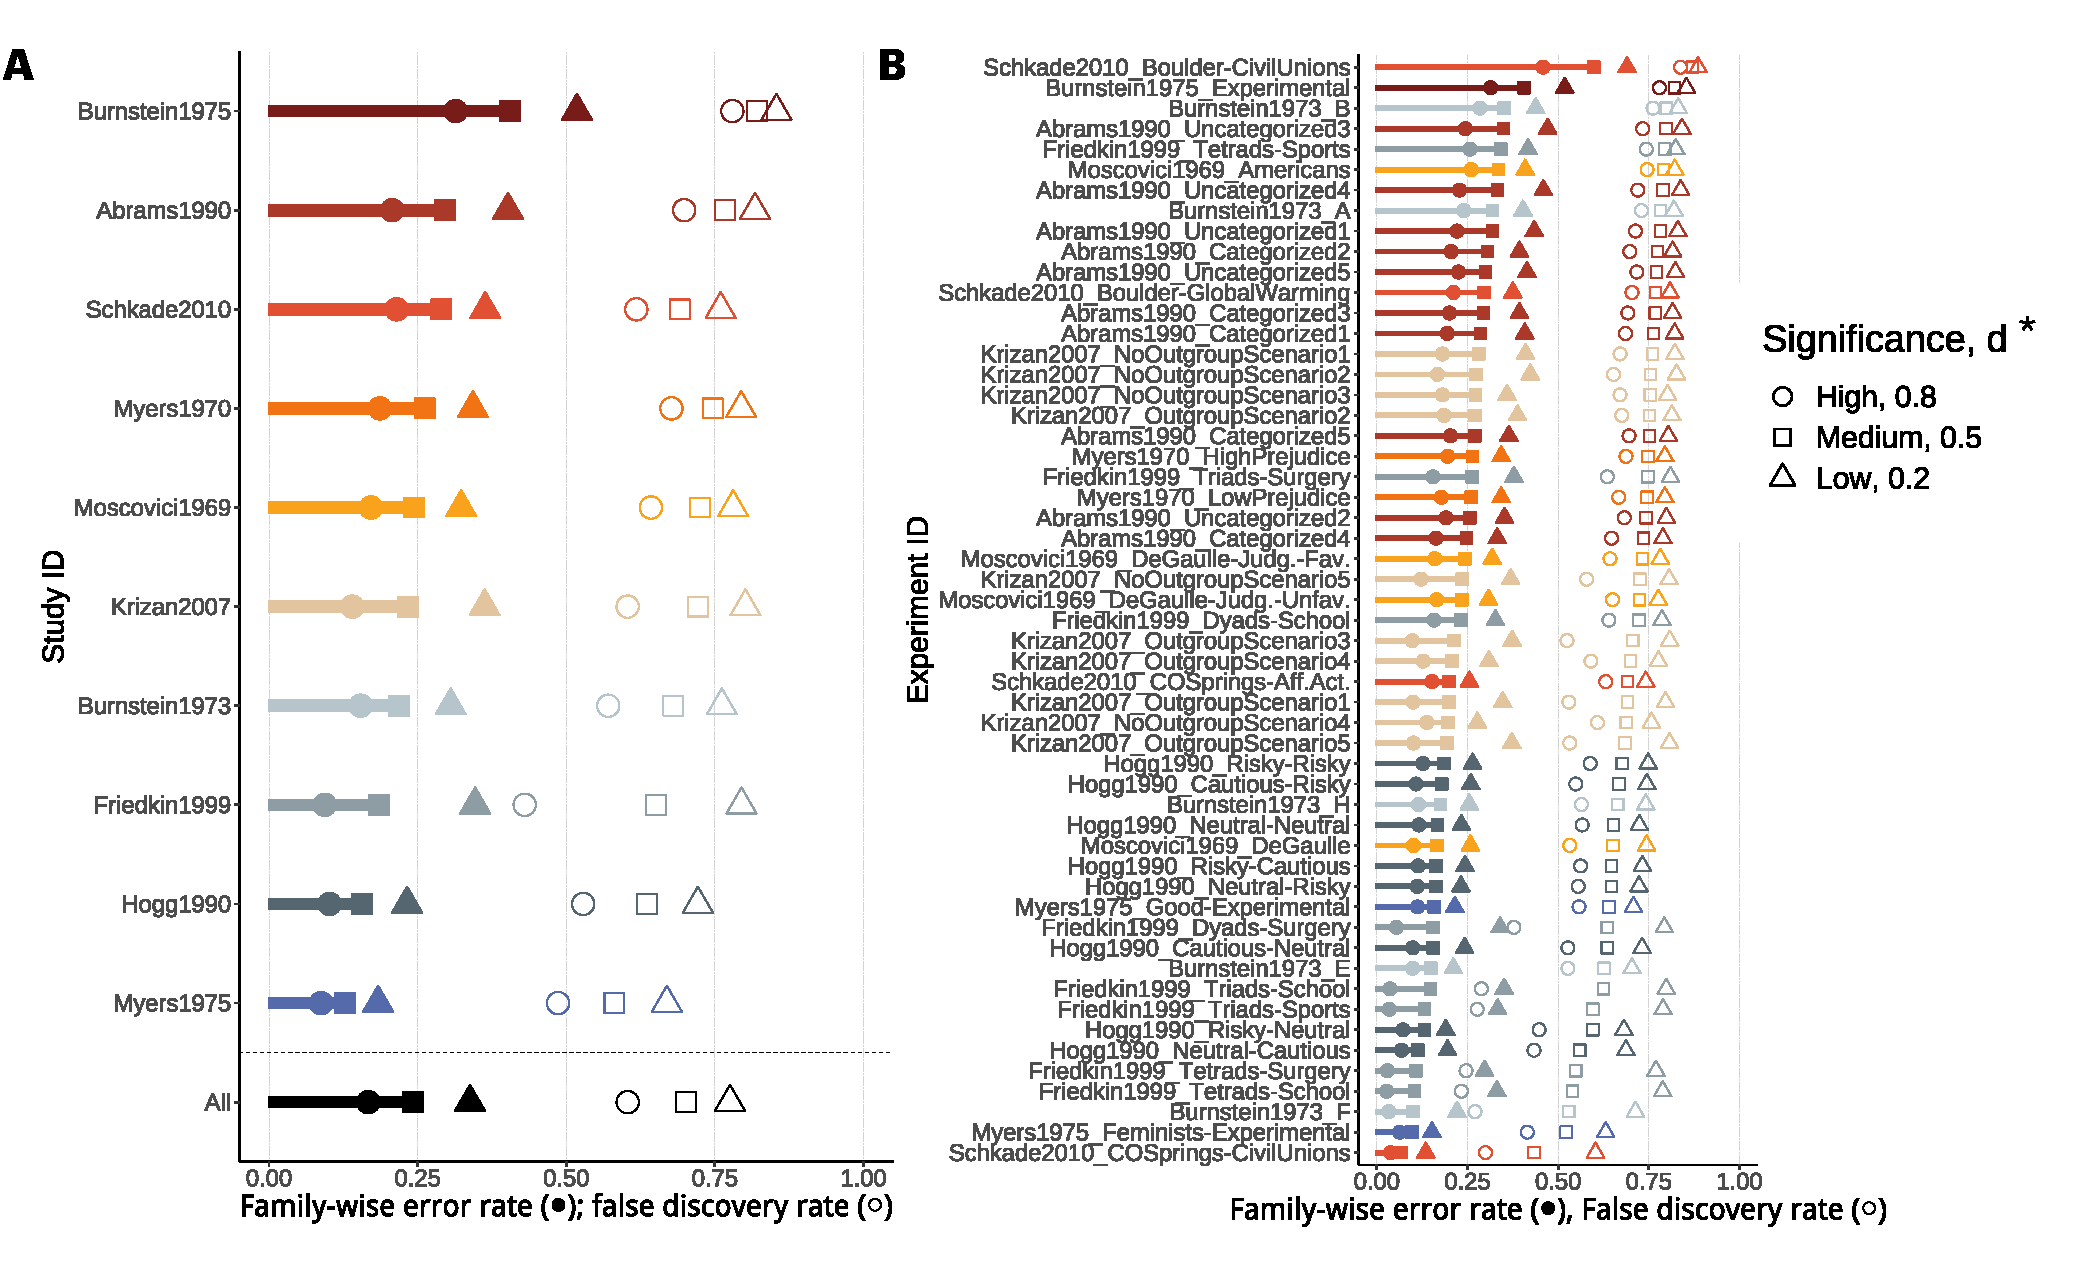
\includegraphics[width=1.1\textwidth]{Figures/Analysis/fwer_fdr_synthesis.pdf}
\end{figure} 

\begin{itemize}
  \item 
    Other $b$ and $W$ values in quantiles.
  \item
    Note that there were many ``significant'' results---in the wrong direction
    (Figure~\ref{fig:OrdinalBoxplot}).
\end{itemize}

\subsection{High significance values ($d^*$) often necessary for FWER of 0.05}

Our simulations can be used a different way, in this case to calculate what
significance value $d^*$ limits the family-wise error rate to the low value of
0.05. 
Solving the inverse problem of which $d^*$ achieves a low family-wise error rate,
which drives the false detection rate. Here we present our calculations to find
$d^*$ that achieve $\alpha(d^*) = 0.05$. 


\begin{figure}
  \caption{
    \textbf{Significance value, $d^*$, to limit family-wise error 
    rate of 0.05 for each identified study.} The Moscovici and Zavalloni (1969)
    ``Americans'' question would require the greatest $d^*$ to achieve $\alpha \leq
    0.05$, even though it does not have the highest error rates. This is because of
    larger outliers in simulated $d$ for this condition compared to others with
    greater error rates (Figure~\ref{fig:OrdinalBoxplot}).
  }
  \centering
    \includegraphics[width=0.75\textwidth]{Figures/Analysis/sigval_for_low_fwer.pdf}
  \label{fig:sigval_for_low_fwer}
\end{figure}

